\section{Inverse Functions} \label{S:inversefunctions}
\setcounter{previewactivity}{0}
%
For this section, we will use the concept of Cartesian product of two sets $A$ and $B$, denoted by $A \times B$, which is the set of all ordered pairs $(x, y)$ where $x \in A$ and $y \in B$.  That is,
\begin{center}
$A \times B = \left\{ { {\left( {x,y} \right)} \mid x \in A\text{ and }y \in B} \right\}.$
\end{center}
See \typeu Activity~\ref*{PA:cartesianproduct} in Section~\ref{S:cartesian} for a more thorough discussion of this concept. 
\begin{previewactivity}[\textbf{Functions and Sets of Ordered Pairs}] \label{PA:functionasordered} \hfill \\
When we graph a real function, we plot ordered pairs in the Cartesian plane where the first coordinate is the input of the function and the second coordinate is the output of the function.  For example, if  $g\x \mathbb{R} \to \mathbb{R}$, then every point on the graph of  $g$  is an ordered pair  $( {x, y} )$ of real numbers where  $y = g( x )$.  This shows how we can generate ordered pairs from a function.  It happens that we can do this with any function.
For example, let  
\[
A = \left\{ {1, 2, 3} \right\} \text{ and } B = \left\{ {a, b} \right\}.
\]
Define the function  $F\x A \to B$ by  
\[
  F( 1 ) = a, \quad  
  F( 2 ) = b, \quad \text{ and} \quad 
  F( 3 ) = b. 
\]

%\[
%\begin{aligned}
%  F( 1 ) &= a, \\ 
%  F( 2 ) &= b,\text{ and} \\ 
%  F( 3 ) &= b. \\ 
%\end{aligned}
%\]
We can convert each of these to an ordered pair in  $A \times B$ by using the input as the first coordinate and the output as the second coordinate.  For example, 
$F( 1 ) = a$ is converted to $( 1, a )$, 
$F( 2 ) = b$ is converted to $( 2, b )$, and 
$F( 3 ) = b$ is converted to $( 3, b )$.  So we can think of this function as a set of ordered pairs, which is a subset of  $A \times B$, and write
\[
F = \left\{ {( {1, a} ), ( {2, b} ), ( {3, b} )} \right\}\!.
\]

\noindent
\note  Since  $F$  is the name of the function, it is customary to use  $F$  as the name for the set of ordered pairs.
%Any function  $f\x A \to B$ can be thought of as a set of ordered pairs that is a subset of  
%$A \times B$.  This subset is
%\begin{multicols}{2}
%$f = \left\{ { {( {a, f( a )} ) } \mid a \in A} \right\}$, \qquad or
% 
%$f = \left\{ {( {a, b} ) \in A \times B   \mid b = f( a )} \right\}$.
%\end{multicols}
%\noindent
%\underline{Note}:  Since  $f$  is the name of the function, it is customary to use  $f$  as the name for the set of ordered pairs.
%\vskip10pt
\noindent
 \begin{enumerate}
\item Let  $A = \left\{ {1, 2, 3} \right\}$ and let  $C = \left\{ {a, b, c, d} \right\}$.  Define the function  $g\x A \to C$ by  $g( 1 ) = a$, $g( 2 ) = b$, and 
$g( 3 ) = d$.  Write the function  $g$  as a set of ordered pairs in  $A \times C$. 
\end{enumerate}
For another example, if we have a real function, such as  $g\x \mathbb{R} \to \mathbb{R}$  by  $g( x ) = x^2  - 2$, then we can think of  $g$  as the following infinite subset of  $\mathbb{R} \times \mathbb{R}$:
\[
g = \left\{ { {( {x, y} ) \in \mathbb{R} \times \mathbb{R}} \mid y = x^2  - 2} \right\}\!.
\]
We can also write this  as 
$g = \left\{ {( {x, x^2 - 2} )} \mid x \in \mathbb{R} \right\}$.  
%\[
%g = \left\{ {( {x, y} )} \mid y = x^2  - 2 \right\} \quad \text{ or } \quad
%g = \left\{ {( {x, x^2 - 2} )} \mid x \in \mathbb{R} \right\}\!.
%\]


\begin{enumerate} \setcounter{enumi}{1}
\item Let $f\x \Z \to \Z$ be defined by $f(m) = 3m +5$, for all $m \in \Z$.  Use set builder notation to write the function $f$ as a set of ordered pairs, and then use the roster method to write the function $f$ as a set of ordered pairs.
\end{enumerate}
So any function  $f\x A \to B$ can be thought of as a set of ordered pairs that is a subset of  $A \times B$.  This subset is
\[
f = \left\{ { {( {a, f( a )} ) } \mid a \in A} \right\} \quad \text{or} 
\quad f = \left\{ {( {a, b} ) \in A \times B   \mid b = f( a )} \right\}\!.
\]

\noindent
On the other hand, if we started with  $A = \left\{ {1, 2, 3} \right\}$, 
$B = \left\{ {a, b} \right\}$, and 
\[
G = \left\{ {( {1, a} ), ( {2, a} ), ( {3, b} )} \right\} \subseteq A \times B ,
\]
then we could think of  $G$  as a function from  $A$  to  $B$  with  $G( 1 ) = a$, $G( 2 ) = a$, and $G( 3 ) = b.$  The idea is to use the first coordinate of each ordered pair as the input, and the second coordinate as the output.  However, not every subset of  $A \times B$ can be used to define a function from  $A$  to  $B$.  This is explored in the following questions.

\setcounter{oldenumi}{\theenumi}
\begin{enumerate} \setcounter{enumi}{\theoldenumi}
\item Let  $f = \left\{ {( {1, a} ), ( {2, a} ), ( {3, a} ), ( {1, b} )} \right\}$. Could this set of ordered pairs be used to define a function from  $A$  to  $B$?  Explain.

\item Let $g = \left\{ {( {1, a} ), ( {2, b} ), ( {3, a} )} \right\}$.  Could this set of ordered pairs be used to define a function from  $A$  to  $B$?  Explain.

\item Let $h = \left\{ {( {1, a} ), ( {2, b} )} \right\}$.  Could this set of ordered pairs be used to define a function from  $A$  to  $B$?  Explain.
\end{enumerate}
\hbreak

\end{previewactivity}


\endinput


\begin{previewactivity}[\textbf{A Composition of Two Specific Functions}] \label{PA:compositionoftwo} \hfill \\
Let  $A = \left\{ {a, b, c, d} \right\}$ and  let  $B = \left\{ {p, q, r, s} \right\}$.

\begin{enumerate}
\item Construct an example of a function  $f\x A \to B$  that is a bijection.  Draw an arrow diagram for this function.

\item On your arrow diagram, draw an arrow from each element of  $B$  back to its corresponding element in  $A$.  Explain why this defines a function  from  $B$  to  $A$.  \label{PA:compositionoftwo2}

\item If the name of the function in Part~(\ref{PA:compositionoftwo2}) is  $g$, so that  
$g\x B \to A$, what are  
$g( p )$, $g( q )$, $g( r )$, and $g( s )$?

\item Construct a table of values for each of the functions $g \circ f\x A \to A$  and  
$f \circ g\x B \to B$. What do you observe about these tables of values?
\label{PA:compositionoftwo4}

%\begin{center}
%\begin{tabular}{c | c  p{0.5in}  c | c   }
%$x$  &  $( {g \circ f} )( x )$  &  & $y$ & 
%$( {f \circ g} )( y )$ \\ \cline{1-2} \cline{4-5}
%$a$  &  &  &  $p$  &  \\ \cline{1-2} \cline{4-5}
%$b$  &  &  &  $q$  &  \\ \cline{1-2} \cline{4-5}
%$c$  &  &  &  $r$  &  \\ \cline{1-2} \cline{4-5}
%$d$  &  &  &  $s$  &  \\ \cline{1-2} \cline{4-5}
%\end{tabular}
%\end{center}

%\item What do you observe about the tables of values in Part~(\ref{PA:compositionoftwo4})?
\end{enumerate}
\end{previewactivity}
\hbreak

\endinput

%
\setcounter{equation}{0}
\setcounter{equation}{0}
\subsection*{The Ordered Pair Representation of a Function}
\index{function!as set of ordered pairs}%
In \typeu Activity~\ref*{PA:functionasordered}, we observed that if we have a function  
$f\x A \to B$, we can generate a set of ordered pairs $f$  that is a subset of  $A \times B$ as follows:
\[
  f = \left\{ { {\left( {a, f( a )} \right)} \mid a \in A} \right\} \quad \text{ or}  
  \quad f = \left\{ {( {a, b} ) \in A \times B \mid b = f( a )} \right\}\!.  
\]
However, we also learned that some sets of ordered pairs cannot be used to define a function.  We now wish to explore under what conditions a set of ordered pairs can be used to define a function.
  Starting with a function $f\x  A \to B$, since  $\text{dom}( f ) = A$, we know that
%
\begin{equation} \label{eq:65a}
\text{For every }  a \in A, \text{ there exists a }  b \in B  \text{ such that }  
( {a, b} ) \in f.
\end{equation}
%
Specifically, we use  $b = f( a )$.  This says that every element of  $A$  can be used as an input.  In addition, to be a function, each input can produce only one output.  In terms of ordered pairs, this means that there will never be two ordered pairs   
$( {a, b} )$  and  $( {a, c} )$  in the function  $f$  where  
$a \in A$, $b, c \in B$, and  $b \ne c$.  We can formulate this as a conditional statement as follows:
\begin{align} 
&\text{For every } a \in A \text{ and every } b, c \in B,  \notag \\
&\text{ if } ( {a, b} ) \in f  \text{ and } ( {a, c} ) \in f, 
\text{ then } b = c. \label{eq:65b}
\end{align}
%
This also means that if we start with a subset  $f$  of  $A \times B$  that satisfies  conditions~(\ref{eq:65a})  and~(\ref{eq:65b}), then we can consider  $f$  to be a function  from  $A$  to  $B$  by using  \linebreak
$b = f( a )$  whenever $( {a, b} )$  is in  $f$.  This proves the following theorem.
\enlargethispage{\baselineskip}
%\hbreak
%
\begin{theorem} \label{T:functionasordered}
Let  $A$  and  $B$  be nonempty sets and let $f$ be a subset of $A \times B$ that satisfies the following two properties:

\begin{itemize}
\item For every  $a \in A$, there exists  $b \in B$  such that  
$( {a, b} ) \in f$\!; and

\item For every  $a \in A$ and every  $b, c \in B$, if  $( {a,\;b} ) \in f$  and  $( {a, c} ) \in f$, then  $b = c$.
\end{itemize}
If we use  $f( a ) = b$ whenever  $( {a, b} ) \in f$, then  $f$  is a function from  $A$  to  $B$.
\end{theorem}
%
\noindent
\textbf{A Note about Theorem~\ref{T:functionasordered}}.    
The first condition in Theorem~\ref{T:functionasordered} means that every element of  $A$  is an input, and the second condition ensures that every input has exactly one output.  Many texts will use Theorem~\ref{T:functionasordered} as the definition of a function.  Many mathematicians believe that this ordered pair representation of a function is the most rigorous definition of a function.  It allows us to use set theory to work with and compare functions.  For example, equality of functions becomes a question of equality of sets.  Therefore, many textbooks will use the ordered pair representation of a function as the definition of a function.
\hbreak
%
\begin{prog}[\textbf{Sets of Ordered Pairs that Are Not Functions}] \label{prog:ordered} \hfill \\
Let  $A = \left\{ {1, 2, 3} \right\}$  and let  $B = \left\{ {a, b} \right\}$.  Explain why each of the following subsets of $A \times B$ cannot be used to define a function from $A$ to $B$.
\begin{multicols}{2}
\begin{enumerate}
\item $F = \left\{ {( {1, a} ), ( {2, a} )} \right\}$.

\item $G = \left\{ {( {1, a} ), ( {2, b} ), ( {3, c} ), ( {2, c} )} \right\}$.
\end{enumerate}
\end{multicols}
\end{prog}
\hbreak
%

\endinput

\subsection*{The Inverse of a Function}
In previous mathematics courses, we learned that the exponential function (with base  $e$) and the natural logarithm function are inverses of each other.  This was often expressed as follows:
\begin{align*}
&\text{For each } x \in \R \text{ with } x > 0 \text{ and for each } y \in \R, \\
&y = \ln x \text{ if and only if } x = e^y.
\end{align*}
Notice that this means that $x$ is the input and $y$ is the output for the natural logarithm function if and only if $y$ is the input and $x$ is the output for the exponential function.  In essence, the inverse function (in this case, the exponential function) reverses the action of the original function (in this case, the natural logarithm function).  In terms of ordered pairs (input-output pairs), this means that if  $( {x, y} )$ is an ordered pair for a function, then  $( {y, x} )$ is an ordered pair for its inverse.  This idea of reversing the roles of the first and second coordinates is the basis for our definition of the inverse of a function.
%\begin{itemize}
%\item For each  $x \in \R$,  if  $y = e^x $, then  $\ln y = x$.
%
%\item For each  $x \in \R$ such that  $x > 0$,  if  $y = \ln x$, then  $e^y  = x$.
%\end{itemize}
%
%In each case,  when  $x$  is the input for one of the functions,  $y$  is the output.  If  $y$  is used as the input for the other function, then this produces  $x$  as the output.   In essence, the inverse function reverses the action of the original function.  In terms of ordered pairs (input-output pairs), this means that if  $( {x, y} )$ is an ordered pair for a function, then  $( {y, x} )$ is an ordered pair for its inverse.  This idea of reversing the roles of the first and second coordinates is the basis for our definition of the inverse of a function.
%
\begin{defbox}{inversefunction}{Let  $f\x A \to B$  be a function.  The \textbf{inverse of}
\index{inverse of a function}%
\index{function!inverse of}%
  $\boldsymbol{f}$\!, denoted by  $f^{ - 1} $,
\label{sym:finverse} is the set of ordered pairs  
$\left\{ { {( {b, a} ) \in B \times A} \mid f( a ) = b} \right\}$.  That is,
\[
f^{ - 1}  = \left\{ { {( {b, a} ) \in B \times A} \mid f( a ) = b} \right\}\!.
\]
If we use the ordered pair representation for  $f$\!, we could also write
\[
f^{ - 1}  = \left\{ { {( {b, a} ) \in B \times A} \mid ( {a, b} ) \in f} \right\}\!.
\]
}
\end{defbox}
%
Notice that this definition does not state that  $f^{ - 1} $  is a function.  It is simply a subset of  $B \times A$.  After we study the material in Chapter~\ref{C:equivrelations}, we will say that this means that  $f^{ - 1}$ is a \textbf{relation} from  $B$  to  $A$.  This fact, however, is not important to us now.  We are mainly interested in the following question:

\begin{center}
\fbox{
\parbox{4.5in}{{\textbf{Under what conditions will the inverse of the function  $\boldsymbol{f\x A \to B}$  be a function from  $B$  to  $A$?}}
}}
\end{center}

\begin{prog}[\textbf{Exploring the Inverse of a Function}] \label{prog:exploringinverse} \hfill \\
Let  $A = \left\{ {a, b, c} \right\}$, $B = \left\{ {a,b,c,d} \right\}$, and 
$C = \left\{ {p, q, r} \right\}$.  Define
\begin{center}
\begin{tabular}{c | c | c}
$f\x A \to C$ by &  $g\x A \to C$ by &  $h\x B \to C$ by \\
$f( a ) = r $  &  $g( a ) = p $  &  $h( a ) = p $ \\
$f( b ) = p $  &  $g( b ) = q $  &  $h( b ) = q $ \\
$f( c ) = q $  &  $g( c ) = p $  &  $h( c ) = r $ \\
                          &                            &  $h( d ) = q $
\end{tabular}
\end{center}
\begin{enumerate}
\item Draw an arrow diagram for each function.  \label{A:exploringinverse1}

\item Determine the inverse of each function as a set of ordered pairs.

\item \begin{enumerate} \item Is  $f^{ - 1} $ a function from  $C$  to  $A$?  Explain.

  \item Is  $g^{ - 1} $ a function from  $C$  to  $A$?  Explain.

  \item Is  $h^{ - 1} $  a function from  $C$  to  $B$?  Explain.
\end{enumerate}
\label{A:exploringinverse3}

\item Draw an arrow diagram for each inverse from  Part~(\ref{A:exploringinverse3}) that is a function.  Use your existing arrow diagram from Part~(\ref{A:exploringinverse1}) to draw this arrow diagram.

\item Make a conjecture about what conditions on a function  $F\x S \to T$ will ensure that its inverse is a function  from  $T$  to  $S$.
\end{enumerate}
\end{prog}
%\hbreak
%
We will now consider a general argument suggested by the explorations in Progress 
Check~\ref{prog:exploringinverse}.  By definition, if  $f\x A \to B$  is a function, then  
$f^{ - 1} $ is a subset of  $B \times A$.  However,  $f^{ - 1} $ may or may not be a function from  $B$  to  $A$.  For example, suppose that  $s, t \in A$ with  $s \ne t$  and  
$f( s ) = f( t )$.  This is represented in 
Figure~\ref{fig:inversenotfunction}.

\begin{figure}[h]
\begin{center}
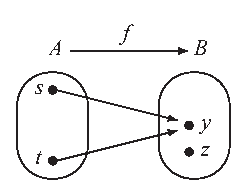
\includegraphics{figps-noinverse.eps}
\caption{The Inverse Is Not a Function} \label{fig:inversenotfunction}
\end{center}
\end{figure}


In this case, if we try to reverse the arrows, we will not get a function from  $B$  to  $A$.  This is because  $( {y, s} ) \in f^{ - 1} $  and  
$( {y, t} ) \in f^{ - 1} $ with  $s \ne t$.  Consequently,  $f^{ - 1} $  is not a function.  This suggests that when  $f$  is not an injection, then  $f^{ - 1} $  is not a function.  

Also, if  $f$  is not a surjection, then there exists a  $z \in B$ such that  
$f( a ) \ne z$ for all  $a \in A$, as in the diagram in 
Figure~\ref{fig:inversenotfunction}.  In other words, there is no ordered pair in  $f$  with  $z$  as the second coordinate.  This means that there would be no ordered pair in  
$f^{ - 1} $  with  $z$  as a first coordinate.  Consequently, $f^{ - 1} $  cannot be a function from  $B$  to  $A$.

This motivates the statement in Theorem~\ref{T:inverseandbijection}.  In the proof of this theorem, we will frequently change back and forth from the input-output representation of a function and the ordered pair representation of a function.  The idea is that if  $G\x S \to T$  is a function, then for  
$s \in S$  and  $t \in T$\!,
\[
G( s ) = t  \text{ if and only if }  ( {s, t} ) \in G.
\]
When we use the ordered pair representation of a function, we will also use the ordered pair representation of its inverse.  In this case, we know that
\[
( {s, t} ) \in G\text{ if and only if }( {t, s} ) \in G^{ - 1}. 
\]
%\hbreak
%
\begin{theorem} \label{T:inverseandbijection}
Let  $A$  and  $B$  be nonempty sets and let  $f\x A \to B$.  The inverse of  $f$ is a function from  $B$  to  $A$  if and only if  $f$  is a bijection.  
%(That is,  $f$  is both one-to-one and onto.)
\end{theorem}
%
\begin{myproof}
Let  $A$  and  $B$  be nonempty sets and let  $f\x A \to B$.  We will first assume that  $f$  is a bijection and prove that  $f^{ - 1} $ is a function from  $B$  to  $A$.  To do this, we will show that  $f^{ - 1} $ satisfies the two conditions of Theorem~\ref{T:functionasordered}.

We first choose  $b \in B$.  Since the function  $f$  is a surjection,  there exists an  
$a \in A$  such that  $f( a ) = b$.  This implies that  
$( {a, b} ) \in f$ and hence that  $( {b, a} ) \in f^{ - 1} $.  Thus, each element of  $B$  is the first coordinate of an ordered pair in  $f^{ - 1} $, and hence  
$f^{ - 1} $  satisfies the first condition of Theorem~\ref{T:functionasordered}.

To prove that  $f^{ - 1} $  satisfies the second condition of Theorem~\ref{T:functionasordered}, we must show that each element of  $B$  is the first coordinate of exactly one ordered pair in  $f^{ - 1} $.  So let  $b \in B$, $a_1 , a_2  \in A$
 and assume that  
\[
( {b, a_1 } ) \in f^{ - 1} \text{ and } ( {b, a_2 } ) \in f^{ - 1} .
\]
This means that  $( {a_1 , b} ) \in f$ and  $( {a_2 , b} ) \in f$.  We can then conclude that
\[
f( {a_1 } ) = b\text{ and }f( {a_2 } ) = b.
\]
But this means that  $f( {a_1 } ) = f( {a_2 } )$.  Since  $f$  is a bijection, it is an injection, and we can conclude that  $a_1  = a_2 $.  This proves that  $b$  is the first element of only one ordered pair in  $f^{ - 1} $.  Consequently, we have proved that  $f^{ - 1} $  satisfies both conditions of Theorem~\ref{T:functionasordered} and hence that  $f^{ - 1} $  is a function from  $B$  to  $A$.
\vskip6pt

We now assume that  $f^{ - 1} $  is a function from  $B$  to  $A$ and prove that  $f$  is a bijection. First, to prove that  $f$  is an injection, we assume that  $a_1 , a_2  \in A$ and that $f( {a_1 } ) = f( {a_2 } )$.  We wish to show that  $a_1  = a_2 $.  If we let  $b = f( {a_1 } ) = f( {a_2 } )$, we can conclude that
\[
( {a_1 , b} ) \in f \text{ and }( {a_2 , b} ) \in f.
\]
But this means that  
\[
( {b, a_1 } ) \in f^{ - 1} \text{ and }( {b, a_2 } ) \in f^{ - 1}. 
\]
Since we have assumed that  $f^{ - 1} $ is a function, we can conclude that  $a_1  = a_2 $.  Hence,  $f$  is an injection.

Now to prove that  $f$  is a surjection, we choose  $b \in B$ and will show that there exists an  $a \in A$ such that  $f( a ) = b$.  Since  $f^{ - 1} $  is a function,  $b$  must be the first coordinate of some ordered pair in  $f^{ - 1} $.  Consequently, there exists an  
$a \in A$  such that
\[
( {b, a} ) \in f^{ - 1} .
\]
Now this implies that  $( {a, b} ) \in f$ and hence that  $f( a ) = b$.  This proves that  $f$  is a surjection.  Since we have also proved that  $f$  is an injection, we conclude that  $f$  is a bijection.
\end{myproof}
\hbreak

\endinput

\subsection*{Inverse Function Notation}
In the situation where  $f\x A \to B$  is a bijection and  $f^{ - 1} $ is a function from  $B$  to  $A$, we can write  $f^{ - 1} \x B \to A$.  In this case, we frequently say that  $f$  is an \textbf{invertible function},
\index{invertible function}%
\index{function!invertible}%
  and we usually do not use the ordered pair representation for either  $f$  or  $f^{ - 1} $.  Instead of writing  
$( {a, b} ) \in f$, we write  $f( a ) = b$, and instead of writing  $( {b, a} ) \in f^{ - 1} $, we write  $f^{ - 1} ( b ) = a$.  Using the fact that  $( {a, b} ) \in f$  if and only if  $( {b, a} ) \in f^{ - 1} $, we can now write  $f( a ) = b$  if and only if  $f^{ - 1} ( b ) = a$.  We summarize this in Theorem~\ref{T:inversenotation}.

\begin{theorem}  \label{T:inversenotation}
Let  $A$  and  $B$  be nonempty sets and let  $f\x A \to B$  be a bijection.  Then 
$f^{ - 1} \x B \to A$ is a function, and for every  $a \in A$ and $b \in B$,
\[
f( a ) = b  \text{ if and only if } f^{ - 1} ( b ) = a.
\]
\end{theorem}
%
%\hbreak
%
\begin{example}[\textbf{Inverse Function Notation}] \hfill \\
\label{exam:inversenotation}%
For an example of the use of the notation in Theorem~\ref{T:inversenotation}, let  $\R^ +   = \left\{ { {x \in \R} \mid x > 0} \right\}$.  Define

\begin{center}
$f\x \R \to \R$  by  $f( x ) = x^3$; and $g\x \R \to \R^ +  $  by  $g( x ) = e^x $.
\end{center}
\vskip10pt
Notice that  $\R^+ $ is the codomain of  $g$.  We can then say that both  $f$  and  $g$  are bijections.  Consequently, the inverses of these functions are also functions.  In fact,
\begin{center}
$f^{ - 1} \x \R \to \R$  by  $f^{ - 1} ( y ) = \sqrt[3]{y}$; and $g^{ - 1} \x \R^ +   \to \R$  by  $g^{ - 1} ( y ) = \ln y$.
\end{center}
%\begin{list}{}
%\item $f^{ - 1} \x \R \to \R$  by  $f^{ - 1} ( y ) = \sqrt[3]{y}$; and
%
%
%\item  
%
%\item $g^{ - 1} \x \R^ +   \to \R$  by  $g^{ - 1} ( y ) = \ln y$.
%
%\end{list}
\vskip10pt
For each function (and its inverse), we can write the result of Theorem~\ref{T:inversenotation} as follows:
\begin{center}
\begin{tabular}{l | l}
\textbf{Theorem~\ref{T:inversenotation}}   &  \textbf{Translates to:}  \\ \hline
For  $x, y \in \R$,  $f( x ) = y$  &  For  $x, y \in \R$,  $x^3  = y$ \\
if and only if  $f^{ - 1} ( y ) = x$.  &  if and only if $\sqrt[3]{y} = x$.  \\
  &  \\
For  $x \in \R, y \in \R^ +  $,  $g( x ) = y$  &  For  
$x \in \R, y \in \R^ +  $,  $e^x  = y$ \\
if and only if  $g^{ - 1} ( y ) = x$.  &  if and only if  $\ln y = x$.  \\
\end{tabular}
\end{center}
\end{example}
%
\hbreak

\endinput

\subsection*{Theorems about Inverse Functions}
The next two results in this section are two important theorems about inverse functions.  The first is actually a corollary of Theorem~\ref{T:inversenotation}.

\begin{corollary} \label{C:inversecomposition}
Let  $A$  and  $B$  be nonempty sets and let  $f\x A \to B$  be a bijection.  Then
\begin{enumerate}
\item For every $x$ in $A$, $\left( f^{ - 1}  \circ f \right)(x) = x$.
\label{C:inversecomposition1}
\item For every $y$ in $B$, $\left( f \circ f^{ - 1}\right)(y) = y$.
\label{C:inversecomposition2}
\end{enumerate}
%\[
%f^{ - 1}  \circ f = I_A \text{  and  } f \circ f^{ - 1}  = I_B 
%\]
%where  $I_A $ is the identity function on  $A$, and  $I_B $ is the identity function on  $B$.
\end{corollary}
%
\begin{myproof}
Let  $A$  and  $B$  be nonempty sets and assume that  $f\x A \to B$  is a bijection. 
%Recall that for every  $x \in A$,  $I_A ( x ) = x$.  
So let  $x \in A$ and let  $f( x ) = y$.  By Theorem~\ref{T:inversenotation}, we can conclude that  $f^{ - 1} ( y ) = x$.  Therefore,
\[
\begin{aligned}
  \left( {f^{ - 1}  \circ f} \right)( x ) &= f^{ - 1} \! \left( {f( x )} \right) \\ 
                                          &= f^{-1}( y ) \\ 
                                          &= x. \\ 
\end{aligned}
\] 
Hence, for each  $x \in A$, $\left( {f^{ - 1}  \circ f} \right)( x ) = x$.

The proof that for each $y$ in $B$, $\left( f \circ f^{ - 1}\right)(y)  = y$ is 
Exercise~(\ref{exer:inversecomposition}).
\end{myproof}
%\hbreak
%
\addtocounter{theorem}{-2}
\begin{example}[\textbf{continued}] \hfill \\
For the cubing function and the cube root function, we have seen that
\begin{center}
For  $x, y \in \R$,  $x^3  = y$  if and only if  $\sqrt[3]{y} = x$.
\end{center}
Notice that
\begin{itemize}
\item If we substitute  $x^3  = y$ into the equation  $\sqrt[3]{y} = x$, we obtain
$\sqrt[3]{{x^3 }} = x$.

\item If we substitute  $\sqrt[3]{y} = x$ into the equation  $x^3  = y$, we obtain 
$\left( {\sqrt[3]{y}} \right)^3  = y$.
\end{itemize}
This is an illustration of Corollary~\ref{C:inversecomposition}.  We can see this by using 
$f\x \R \to \R$  defined by  $f( x ) = x^3 $ and   
$f^{ - 1} \x \R \to \R$  defined by  $f^{ - 1} ( y ) = \sqrt[3]{y}$.   Then  
$f^{ - 1}  \circ f\x \R \to \R$ and $f^{ - 1}  \circ f = I_\R $.  So for each $x \in \R$,
\[
\begin{aligned}
  \left( {f^{ - 1}  \circ f} \right)( x ) &= x \\ 
      f^{ - 1} \! \left( {f( x )} \right) &= x \\ 
         f^{ - 1} \!\left( {x^3 } \right) &= x \\ 
                         \sqrt[3]{{x^3 }} &= x. \\ 
\end{aligned}
\]
Similarly, the equation  $\left( {\sqrt[3]{y}} \right)^3  = y$ for each  $y \in \R$ can be obtained from the fact that for each $y \in \R$,  $(f \circ f^{ - 1})(y) = y$.
\end{example}
\hbreak
%
\addtocounter{theorem}{1}
%

We will now consider the case where  $f\x A \to B$  and  $g\x B \to C$  are both bijections.   In this case,  $f^{ - 1} \x B \to A$  and  $g^{ - 1} \x C \to B$.  
Figure~\ref {fig:bijectioncomposition} can be used to illustrate this situation.
\begin{figure}[h]
\begin{center}
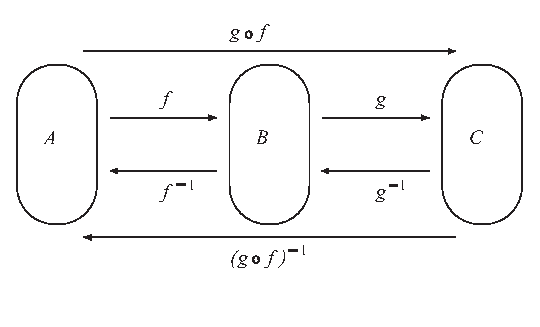
\includegraphics{figps-compinverse.eps}
\caption{Composition of Two Bijections} \label{fig:bijectioncomposition}
\end{center}
\end{figure}

%
By Theorem~\ref{T:compositefunctions},  $g \circ f\x A \to C$  is also a bijection. Hence, by Theorem~\ref{T:inverseandbijection},  
$( {g \circ f} )^{ - 1} $ is a function and, in fact, 
$( {g \circ f} )^{ - 1} \x C \to A$.  Notice that we can also form the composition of  $g^{ - 1} $  followed by  $f^{ - 1} $ to get  $f^{ - 1}  \circ g^{ - 1} \x C \to A$.  Figure~\ref {fig:bijectioncomposition} helps illustrate the result of the next theorem.
%
\setcounter{equation}{0}
\begin{theorem} \label{compositionofbijections}
Let $f\x A \to B$  and  $g\x B \to C$  be bijections.  Then  $g \circ f$  is a bijection and  
$( {g \circ f} )^{ - 1}  = f^{ - 1}  \circ g^{ - 1} $.
\end{theorem}
%
\begin{myproof}
Let $f\x A \to B$  and  $g\x B \to C$  be bijections.  Then  $f^{ - 1} \x B \to A$  and  
$g^{ - 1} \x C \to B$.  Hence, $f^{ - 1}  \circ g^{ - 1} \x C \to A$.  Also, by Theorem~\ref{T:compositefunctions},  $g \circ f\x A \to C$  is a bijection, and hence 
$( {g \circ f} )^{ - 1} \x C \to A$.   We will now prove that for each  
$z \in C$, 
$( {g \circ f} )^{ - 1} ( z ) = ( {f^{ - 1}  \circ g^{ - 1} } )( z )$.

Let  $z \in C$.  Since the function  $g$  is a surjection, there exists a  $y \in B$ such that
\begin{equation} \label{eq:compofbij1} 
g( y ) = z.
\end{equation}
%
Also, since  $f$  is a surjection, there exists an  $x \in A$  such that
\begin{equation} \label{eq:compofbij2}
f( x ) = y.
\end{equation}
%
Now these two equations can be written in terms of the  respective inverse functions as
\begin{align}
g^{ - 1} ( z ) &= y; \text{ and }  \label{eq:compofbij3}\\
f^{ - 1} ( y ) &= x.  \label{eq:compofbij4}
\end{align}
%
Using equations~(\ref{eq:compofbij3}) and~(\ref{eq:compofbij4}), we see that
\begin{align}  \notag
  \left( {f^{ - 1}  \circ g^{ - 1} } \right)( z ) &= f^{ - 1} \left( {g^{ - 1} ( z )} \right) \\ \notag
                                                  &= f^{ - 1} ( y ) \\ \label{eq:compofbij5}                                                  &= x. \\  \notag
\end{align} 
%
Using equations~(\ref{eq:compofbij1}) and~(\ref{eq:compofbij2})  again, we see that  
$( {g \circ f} )( x ) = z$.  However, in terms of the inverse function, this means that
\begin{equation} \label{eq:compofbij6}
( {g \circ f} )^{ - 1} ( z ) = x.
\end{equation}
%
Comparing equations~(\ref{eq:compofbij5}) and~(\ref{eq:compofbij6}), we have shown that for all  $z \in C$,
\linebreak 
$( {g \circ f} )^{ - 1} ( z ) = ( {f^{ - 1}  \circ g^{ - 1} } )( z )$.  This proves that  
$( {g \circ f} )^{ - 1}  = f^{ - 1}  \circ g^{ - 1} $.
\end{myproof}
\hbreak

\endinput

%\subsection*{Construction of the Inverse of a Real Function}


\endinput


\endinput

%
%
%
\begin{activity}[Construction and Existence of Inverse Functions]\label{A:constructinverse}\hfill \\
\index{inverse of a function!construction}%
If $f\x A \to B$ is a bijection, then we know that its inverse is a function.  If  we are given a formula for the function  $f$, it may be desirable to determine a formula for the function  $f^{ - 1} $.  This can sometimes be done, while at other times it is very difficult or even impossible.
\vskip10pt
\noindent
\textbf{Construction of an Inverse Function} \\
Let  $f\x \R \to \R$ be defined by  $f( x ) = 2x^3  - 7$.

\begin{enumerate}
\item Sketch a graph of this function and use the graph to explain why the function is a bijection (one-to-one and onto).  A formal proof is not required.
\end{enumerate}

One way to attempt to find a formula for the inverse of this function is to set  
$y = f( x )$ and solve for  $x$.  In this case, we are using  $x$  for the input of  $f$  and  $y$  for the output of  $f$.  By solving for  $x$  in terms of  $y$, we are attempting to write a formula where   $y$  is the input and  $x$  is the output.  This formula represents the inverse function.

\begin{enumerate}
\setcounter{enumi}{1}
\item Solve the equation  $y = 2x^3  - 7$ for  $x$.  Use this to write a formula for  
$f^{ - 1} ( y )$, where  $f^{ - 1} \x \R \to \R$.  \label{A:constructinverse2}

\item Use the result of Part~(\ref{A:constructinverse2}) to verify that for each  
$x \in \R$,  $f^{ - 1} \!\left( {f( x )} \right) = x$ and for each  
$y \in \R$,  $f \!\left( {f^{ - 1} ( y )} \right) = y$.

\end{enumerate}

\noindent
\note  If we write  $y = f( x )$ for the function  $f$, we are using  $x$  as the independent variable (input) and  $y$  as the dependent variable (output).  In the case where  $f^{ - 1} $ is a function, we may write  $x = f^{ - 1} ( y )$, where  $y$  is the independent variable for  
$f^{ - 1} $.  However, when we are using real functions, we frequently want to graph them.  So we traditionally write each function as a function of  $x$.  
%Even if we have 
%\[
%f^{ - 1} ( y ) = \sqrt[3]{{\frac{{y + 7}}{2}}}, 
%\]
%we will frequently write 
%\[
%f^{ - 1} ( x ) = \sqrt[3]{{\frac{{x + 7}}{2}}}.
%\]
\vskip6pt
\noindent
\textbf{Existence of an Inverse Function}\index{inverse of a function!existence} \\
In calculus we learned that a function  $G$  is an  \textbf{increasing function}
\index{increasing function}%
\index{function!increasing}%
 provided that  
$G( {x_2 } ) > G( {x_1 } )$  whenever  $x_2  > x_1 $.  We also learned that a differentiable function  $G$  is increasing on an interval provided that  
$G'( x ) > 0$ for all  $x$  in that interval.

\begin{enumerate} \setcounter{enumi}{3}
\item Explain why an increasing function is a one-to-one function or an injection.
\end{enumerate}

\noindent
Let  $g\x \R \to \R$ be defined by  $g( x ) = x^3  + x - 5$.

\enlargethispage{\baselineskip}
\begin{enumerate}
\setcounter{enumi}{4}
\item Use  $g'( x )$ to show that $g$ is an injection, and use a graph of  $g$  to show that  $g$  is a surjection.  Explain why this proves the existence of an inverse function  
$g^{ - 1} \x \R \to \R$.

\item If  $y = g( x )$ and hence $y = x^3  + x - 5$, do you think it is possible to solve this equation for  $x$  to obtain a formula for  $g^{ - 1} ( y )$?  Explain.
\end{enumerate}
\end{activity}
\hbreak
%
\begin{activity}[The Inverse Sine Function] \label{A:inversesine} \hfill \\
In order to obtain an inverse function, it is sometimes necessary to restrict the domain (or the codomain) of a function.

\begin{enumerate}
\item Let  $f\x \R \to \R$ be defined by  $f( x ) = \sin x$.  Explain why the inverse of the function  $f$  is not a function.  (A graph may be helpful.)  \label{A:inversesine1}
\end{enumerate}

Notice that if we use the ordered pair representation, then the sine function can be represented as
\[
f  = \left\{ { {( {x, y} ) \in \R \times \R } \mid y = \sin x} \right\}\!.
\]
If we denote the inverse of the sine function by  $\sin ^{ - 1} $, then
\[
f^{ - 1}  = \left\{ { {( {y, x} ) \in \R \times \R } \mid y = \sin x} \right\}\!.
\]
Part~(\ref{A:inversesine1}) proves that  $f^{ - 1} $  is not a function.  However, in previous mathematics courses, we frequently used the ``inverse sine function.''  This is not really the inverse of the sine function as defined in Part~(\ref{A:inversesine1}) but, rather, it is the inverse of the \linebreak
\vspace{2pt}
\noindent
sine function \textbf{restricted to the domain}  
$\left[ {-\dfrac{{\pi }}{2}, \dfrac{\pi }{2}} \right]$.

\begin{enumerate}
\setcounter{enumi}{1}
\item Explain why the function  
$F\x \left[ {- \dfrac{{\pi }}{2}, \dfrac{\pi }{2}} \right] \to \left[ { - 1, 1} \right]$
defined by 
$F( x ) = \sin x$ is a bijection.  \label{A:inversesine2}
\end{enumerate}

The inverse of the function in Part~(\ref{A:inversesine2}) is itself a function and is called the \textbf{inverse sine function}
\index{inverse sine function}%
 (or sometimes the \textbf{arcsine function}).
\index{arcsine function}%

\begin{enumerate}
\setcounter{enumi}{2}
\item What is the domain of the inverse sine function?  What are the range and codomain of the inverse sine function?
\end{enumerate}
%
Let us now use  $F ( x ) = \text{Sin} ( x )$ 
\label{sym:restrictsine} to represent the restricted sine function in Part~(\ref{A:inversesine2}).  Therefore, 
$F^{-1} ( x ) = \text{Sin}^{ - 1} ( x ) $
\label{sym:inversesine}  can be used to represent the inverse sine function.  Observe that
\[
F\x \left[ -{\frac{{\pi }}{2}, \frac{\pi }{2}} \right] \to \left[ { - 1, 1} \right]
	\text{ and }	
F^{ - 1} \x \left[ { - 1, 1} \right] \to \left[ -{\frac{{\pi }}{2}, \frac{\pi }
{2}} \right].
\]
%
\begin{enumerate}
\setcounter{enumi}{3}
\item Using this notation, explain why
\begin{list}{}
\item $\text{Sin}^{ - 1} y = x	\text{ if and only if }	
\left[ {y = \sin x\text{  and  } -\dfrac{{\pi }}{2} \leq x \leq \dfrac{\pi }
{2}} \right]$;

\item $\text{Sin} \!\left( \text{Sin}^{-1} ( y ) \right) = y$ for all 
$y \in \left[ -1, 1 \right]$; and
\item $\text{Sin}^{-1} \!\left( \text{Sin} ( x ) \right) = x$ for all 
$x \in \left[ - \dfrac{\pi}{2}, \dfrac{\pi}{2} \right]$.
\end{list}
\end{enumerate}
\hbreak


\end{activity}

\endinput

\begin{center}
\setlength{\unitlength}{0.3cm}
\begin{picture}(14,10)
\put(2,4){\oval(4,6)}
\put(10,4){\oval(4,6)}

\put(2,2){\circle*{.5}}
\put(2,6){\circle*{.5}}

\put(9.7,4){\circle*{.5}}
\put(9.7,2.5){\circle*{.5}}

\put(1,1.8){$t$}
\put(1,5.8){$s$}
\put(10.4,3.8){$y$}
\put(10.4,2.3){$z$}

\put(1.8,8){$A$}
\put(10,8){$B$}

\put(3,8.2){\vector(1,0){6.6}}
\put(6,8.8){$f$}

\put(2.2,2){\vector(4,1){6.8}}
\put(2.2,6){\vector(4,-1){6.8}}

\end{picture}



\begin{center}
\setlength{\unitlength}{0.5cm}
\begin{picture}(22,10)
\put(2,5){\oval(3,6)}
\put(10,5){\oval(3,6)}
\put(18,5){\oval(3,6)}

\put(1.5,5){$A$}
\put(9.5,5){$B$}
\put(17.5,5){$C$}

\put(4,6){\vector(1,0){4}}
\put(12,6){\vector(1,0){4}}
\put(8,4){\vector(-1,0){4}}
\put(16,4){\vector(-1,0){4}}

\put(6,6.5){$f$}
\put(14,6.5){$g$}
\put(6,3){$f^{ - 1}$}
\put(14,3){$g^{-1}$}

\put(3,8.5){\vector(1,0){14}}
\put(17,1.5){\vector(-1,0){14}}

\put(8.5,9){$g \circ f$}
\put(8.5,0.5){$( g \circ f )^{-1}$}

\end{picture}
\end{center}

\end{center}
